\documentclass[12pt, letterpaper]{article}
\setcounter{tocdepth}{2}
\usepackage[utf8]{inputenc}
\usepackage{hyperref}
\usepackage{xcolor}
\hypersetup{
colorlinks = true,
linkcolor = {black},
urlcolor = {blue},
}
\usepackage{epsfig, url}
\usepackage{epstopdf}
\usepackage{graphicx}
\usepackage{datetime}
\usepackage{multirow}

%\usepackage{wrapfig}
%\usepackage{amsmath}
\usepackage{amssymb}
\usepackage{geometry} 
\geometry{a4paper}              

\usepackage{titling}
\usepackage{tabto}

\setlength{\evensidemargin}{0in}
\setlength{\oddsidemargin}{0in}
\setlength{\textwidth}{6.5in}
\setlength{\textheight}{9.0in}
\setlength{\topmargin}{0in}
\setlength{\headheight}{0in}
\setlength{\headsep}{0in}
\setlength{\itemsep}{-\parsep}



\begin{document}
\title{\large People Oriented Computing Assignment 1\\[0.5cm]
        \bf\Large Analysis of Covid Vaccination Data Visualizations}
\author{\large Luc Aggett, Mert Erol}
\date{October 27th, 2021}
\makeatletter
    \begin{titlepage}
        \begin{center}
        \vbox{}\vspace{5cm}
            {\@title }\\[3cm] 
            {\@author}\\
            %{Instructor: \bf instructor name}\\
            \vfill 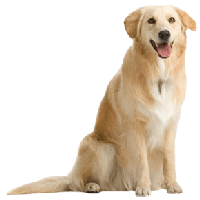
\includegraphics[scale=0.3]{images/logo.png}\\[1cm]
            {\@date}
        \end{center}
    \end{titlepage}
\makeatother
%\thispagestyle{empty}


\newpage
\tableofcontents
\newpage
%\listoftables
\listoffigures
\newpage

\section{Visualisation 1}
\begin{figure}[h]
    \centering
    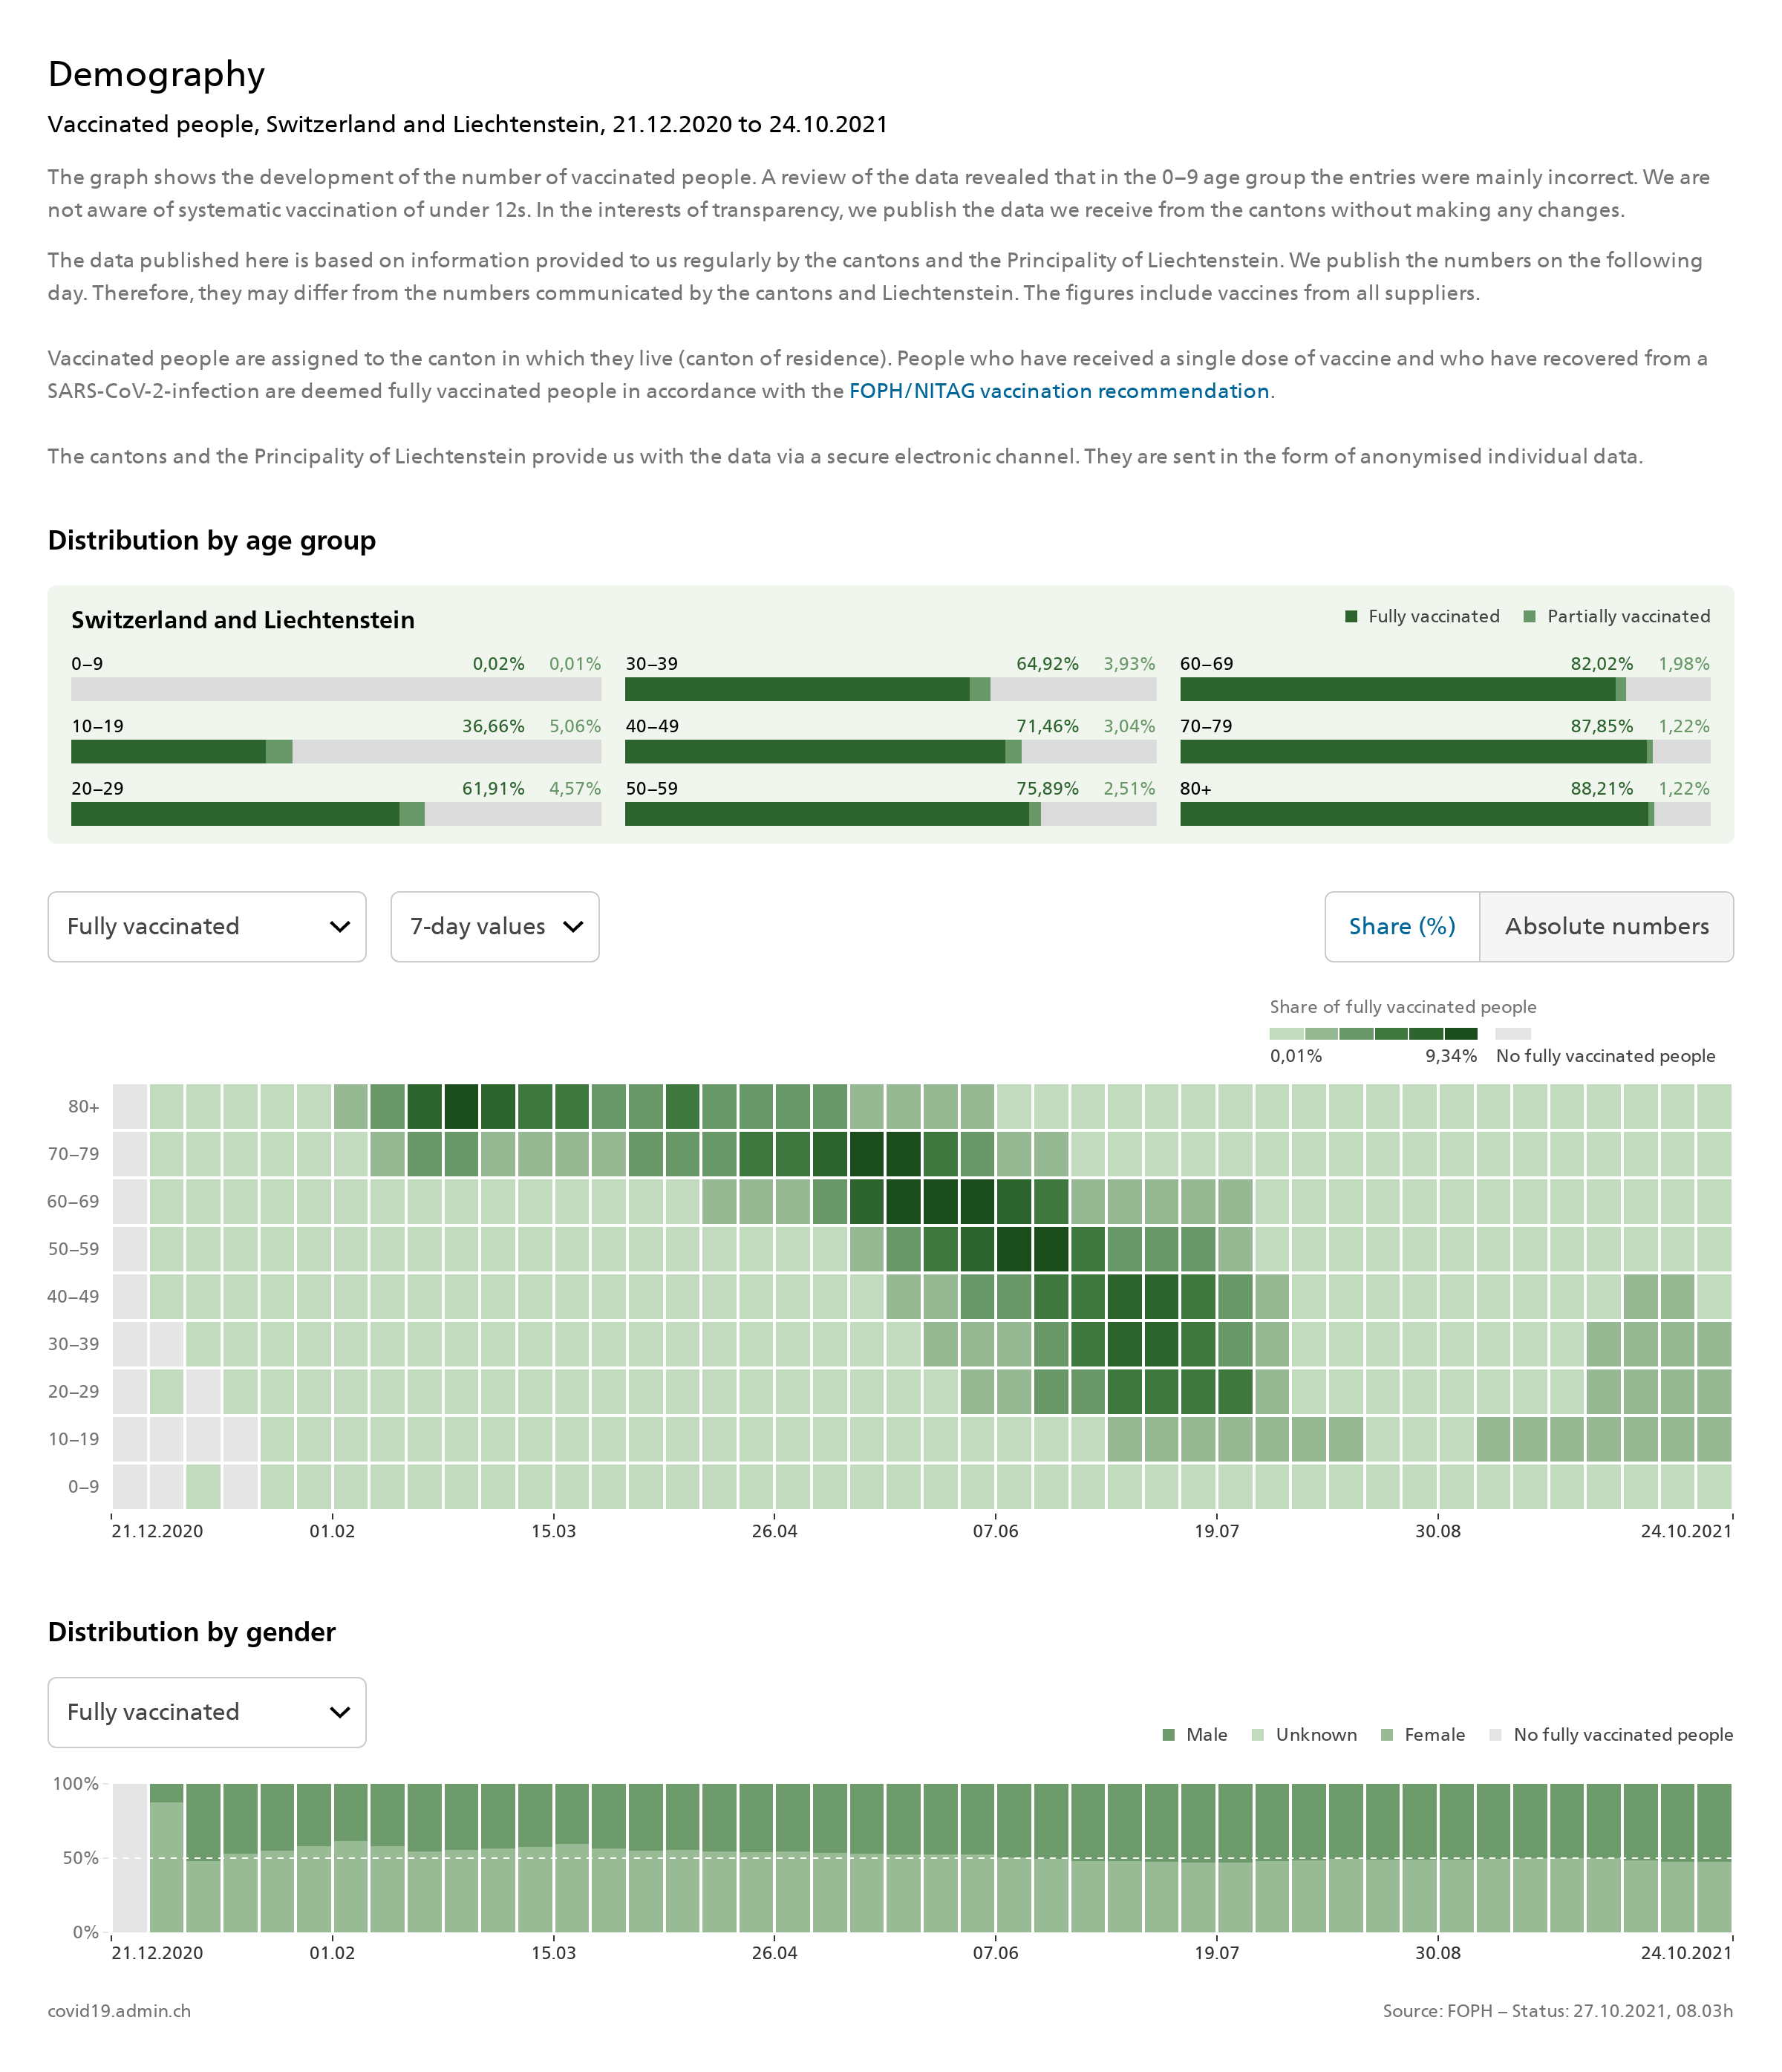
\includegraphics[width=410pt]{images/vis1_3.png}
    \caption{\href{https://www.covid19.admin.ch/en/vaccination/persons}{FOPH Covid19 - Demography}}
    \label{fig:my_label}
\end{figure}
\newpage

\subsection{Description}
This graphic from the Swiss Federal Office for Public Health (Henceforth FOPH) shows the amount of vaccinated people in Switzerland over time, as well as the gender and age distributions of those people. The graph is frequently updated, with the last update at time of writing being on 24.10.2021. The visualisation is split into 2 major parts: Distribution by age group and distribution by gender. the topmost graph shows the distribution of fully vaccinated/partially vaccinated/nonvaccinated people among particular age groups. The second graphic shows the evolution of this data over time. the third graphic shows the distribution by gender.
\subsection{Principles for good design}
\subsubsection{Discoverability}
This Visualisation has additional pieces of information, that are present in the visualisation but not easily discoverable by the user. The first graphic does not provide any extra information to the user when hovered over, but the second and third one do. This could be confusing to a user, or cause them to miss the functionality completely. We only discovered the more detailed view when hovering by accident, while scrolling through the page. An explicit signifier to show the ability to hover over the elements might lead to better discoverability.

\subsubsection{Feedback}
Feedback is provided to the user immediately after changing any of the values, as the graphics change to reflect the selected dataset. The graphics update instantly after any change. The Visualization provides adequate and timely feedback for the user.

\subsubsection{Affordances}
The Visualization affords the selection of multiple criteria, changing which data is presented to the user. The buttons in the UI afford clicking, which reveals a submenu. Some graphic also allow a user to hover over them to receive additional information.


\subsubsection{Constraints}
The amount of interaction in the visualisation is limited, so the user is constrained enough that it is impossible to make an "incorrect" input. All possible user inputs (via standard methods) are accounted for. Interaction and customization are limited in exchange for better ease of use and accessibility. This is important for graphics of this kind, since they are meant to readable by a wider public.
\newpage
\subsubsection{Signifiers}
The current selected dataset is displayed via highlighting for the Share (\%) and Absolute numbers selection. The presence of additional options is signified using a selection box, which is an element familiar to most users. The graphic is slightly unclear in what the options change, since one of the selection boxes causes a complete change in the way the data is displayed - the choice between "7-day" and "Total" options changes the data display from boxes with color saturation indicating the amount of people vaccinated to a graph.
\begin{figure}[h]
    \centering
    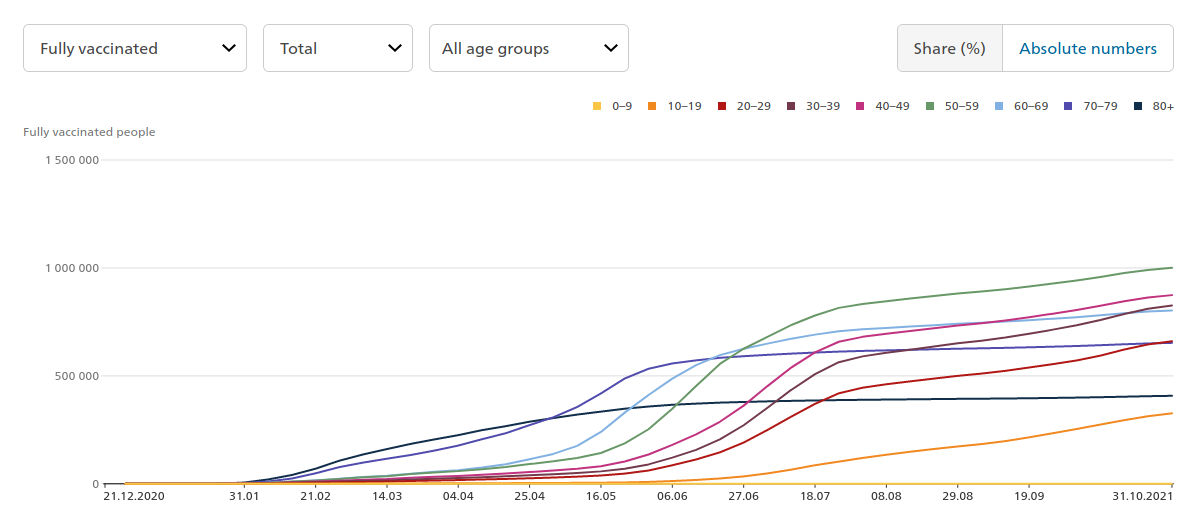
\includegraphics[width=400px]{images/Screenshot_20211106_140017.png}
    \caption{alternate display method for the data if "total" is selected}
    \label{fig:my_label}
\end{figure}

\subsection{Information Visualisation Principles}
\subsubsection{Elementary Graphical Perception (Cleveland and McGill)}
The Visualization mainly uses position and length to represent the data. These are very accurately perceptible according to elementary graphical perception. This helps the visualization to be easily readable.
\subsubsection{Infovis Principles from Edward Tufte}
\textbf{Graphical Integrity:} \\
In the distribution by age group graphic, the size of the bars corresponds directly to the percentage of people they represent. Although this fulfills a part of Tufte's principles of graphical integrity, it fails in Clear, detailed and thorough labeling, since what the size of the bars represents is not clearly conveyed - there are two percentile numbers, but there are 3 values (vaccinated, one dose and unvaccinated) that are represented by the graph. The rest of the graphics are well-labeled. The entire visualisation has a high data density, particularly the distribution by age group graphic, since it implements small multiples, which Tufte says is a great way to visualize large quantities of data. The "7-day" option (the default) also has a very high data density.
\subsection{Interaction Models}
\subsubsection{GOMS Model}
In the GOMS model, we can map a user interacting with the visualization: \\
\textbf{Goals:} The user wants to find out the current percentage of 20-29 year olds that are vaccinated or partially vaccinated \\
\textbf{Operators:} The user needs to scroll down the page of the site to find the relevant graphic. \\
\textbf{Methods:} The user can scroll down the page, or use a search function (CTRL-F, etc) to find the information on the site. \\
\textbf{Selection Rules: } Depending on the users familiarity with the website, they may scroll down to the point where the data is located, or they may have to search the site. \\
\\
From this analysis using the GOMS model, we can see that the Visualization may need a more clear way of navigating the information presented on the site. Having a sidebar denoting the current dataset / showing a list of the datasets would help make it easier to find content on the site.



\newpage

\section{Visualisation 2}
\begin{figure}[h]
    \centering
    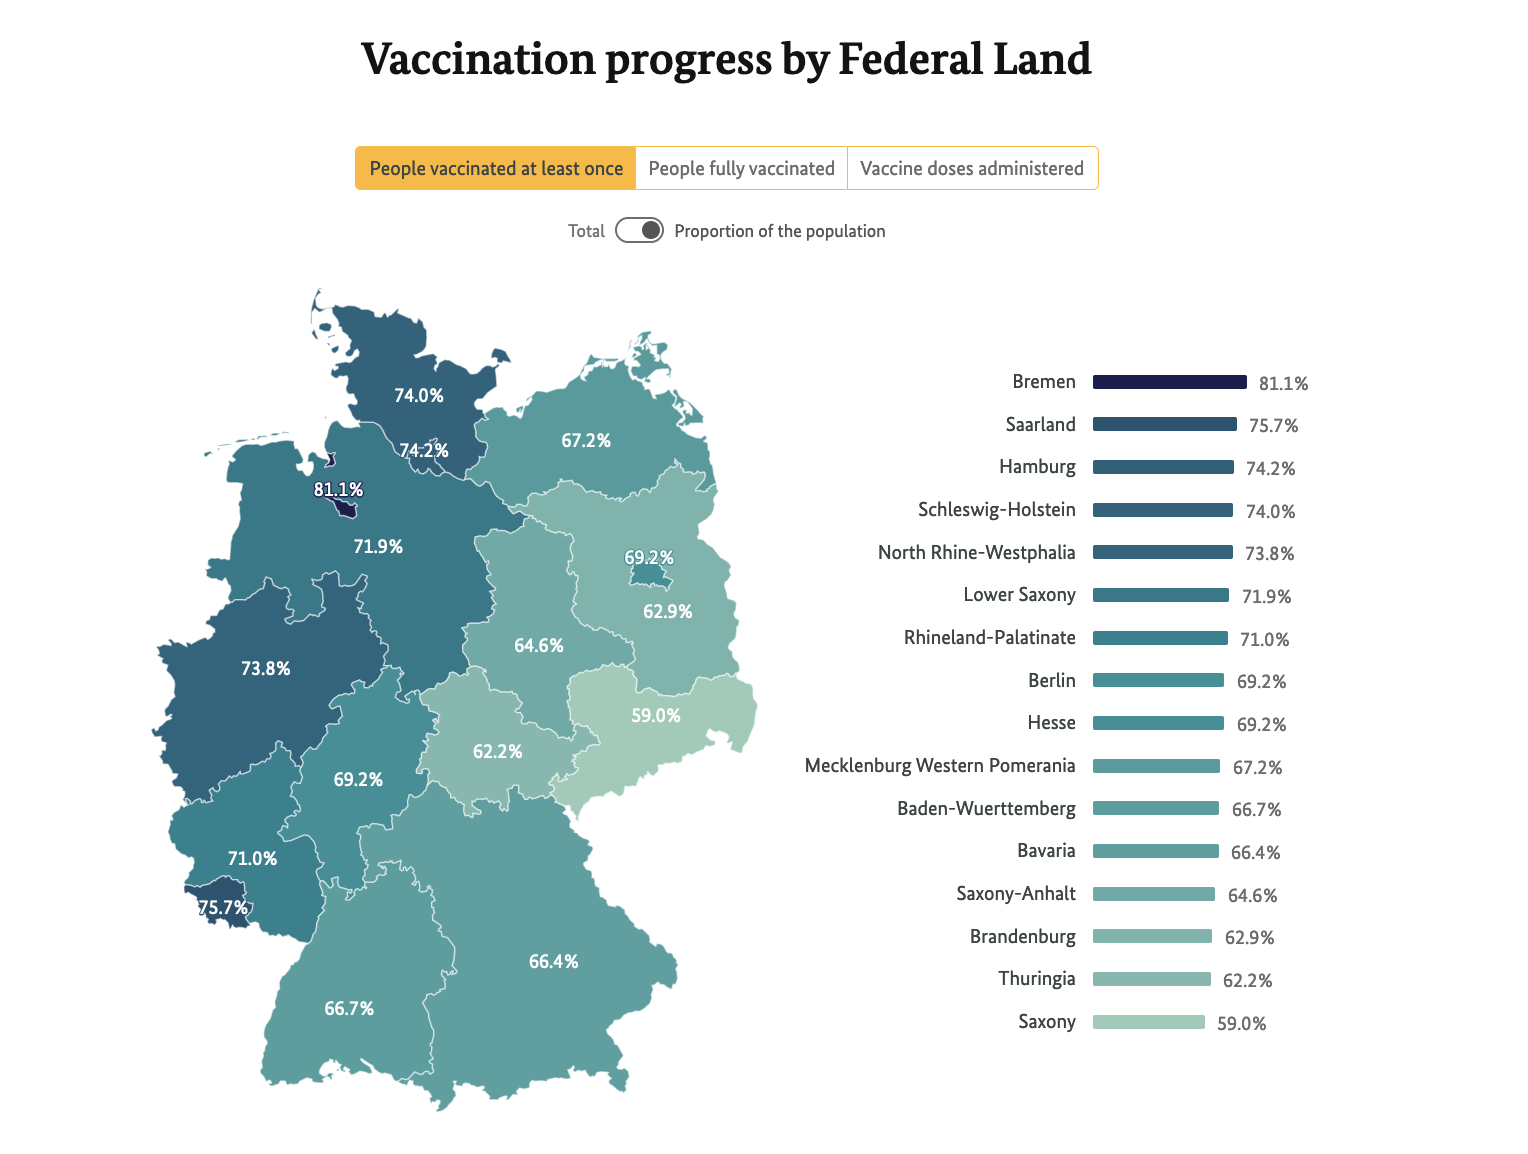
\includegraphics[width=410pt]{images/Impfdashboard.png}
    \caption{\href{https://impfdashboard.de/en/}{Vaccination progress by Federal Land}}
    \label{fig:my_label}
\end{figure}
\subsection{Description}
Impfdashboard is a website created by the German Federal Ministry of Health to visualize the current state of vaccines focused on their country. Many different forms of visualizations are presented by the ministry such as vaccination progress by federal land, progress by age groups, daily deliveries and much more. Every visualization is fully interactive and shows more information or changes design depending on the way the user hovers the cursor over a spot in a graph or clicks on certain buttons. 

\subsection{Principles for good design}
The design of the website is pretty unique and has to be addressed and discussed as it clearly uses the important principles for good design.
Focusing on usability first, the user can clearly tell that the way the visualizations are set up is top notch. The structure of the site is clear and invites the user to hover over graphs and scroll through the page to discover more information with each click of a button or hovering over certain spots. But what is more important than usability in case of COVID-vaccines? - Usefulness. All the information provided proves useful as the information on vaccination data might help us predict the further steps are going to be taken during the fight against COVID-19.

\subsubsection{Affordances}
Starting with affordances we will begin analyzing the important principles of good design. The visualization of the data affords the user to choose the type of data the user wants to see by scrolling through the page and stopping at the chosen visualization. Furthermore, the user can switch between sub menus of each visual if provided by clicking on the labeled buttons.

\subsubsection{Signifiers}
In general the website does not have that many signifiers but rather prompts the user to “discover” the affordances by themselves by highlighting certain parts of the visuals or text when hovered over. Some affordances are backed up by signifiers that are written text inside boxes.

\subsubsection{Constraints}
The way each visualization is designed is pretty simple and doesn't allow for further interactions except for small sets of data shown by hovering over parts that the user wants to receive further information on. There might be possible cultural constraints if the user does not know the map of Germany or how each federal land handles the vaccination since there is no information shown regarding the laws. The way that dates are displayed may also lead to a cultural restriction as some countries or cultures use a different way of describing dates of the year.

\subsubsection{Mapping}
The focus of each data set is set on Germany and its Federal lands. The data for individual lands is displayed when the user hovers the mouse on the according land on the map. In the visualization for vaccination progress in each federal land the user can switch through data sets regarding people vaccinated once, people fully vaccinated and the amount of vaccines administered. All relevant information is well grouped which helps to create a clean and easily understandable dashboard.

\subsubsection{Feedback}
The way the website communicates with the user is direct and seamless. As soon as the user hovers their mouse over parts of a visualization there is an immediate reaction by the website to provide detailed information regarding percentages and numbers.

\subsubsection{Discoverability}
Some of the signifiers and affordances mentioned above are not visible at first but then become largely intuitive as soon as the user moves their mouse. The combination of this and the immediate feedback make sure that the page has great discoverability. The decision of making certain things invisible at first makes sure the website has great readability while still providing detailed data if the user wishes to see them.


\subsection{Information Visualisation Principles}
\subsubsection{Infovis Principles from Edward Tufte}

\textbf{Data Graphics:}
Impfdashboard follows the principles of data graphics very well. The page shows all the relevant data while still being able to minimize non-data-ink. The page is able to erase non-data-ink by using a plain white background and making sure that all the relevant data is in an easily readable and visible color.
Impfdashboard also uses the principles for a friendly data graphic. Words run from left to right, when a user hovers over certain areas in the graphics small text boxes appear to help explain the data and because the color palette is chosen in a certain way, nearly everyone can perceive the differences in color. One element of the page that could be seen as a disadvantageous is the way the first thing you see on the page is written in a larger font which makes reaching the data the user wants to see take a bit longer than some might want.

\subsection{Interaction Models}
\subsubsection{Seven stage model}
\begin{itemize}
    \item\textbf{Goal:}
    Find information on vaccination data inside Germany.
    \item\textbf{Forming the intention:}
    Visit Impfdashboard and look at the data
    \item\textbf{Specifiying the Action:}
    Devise a plan to enter the URL into the users browser and visit the page to read the data.
    \item\textbf{Executing the Action:}
    Executing the action of entering the URL into the browser, visiting the page and reading the data provided by the Ministry of Health.
    \item\textbf{State of the World:}
    The browser now loads and shows the main page of Impfdashboard with all the visualizations.
    \item\textbf{Perceiving the state of the World:}
    User physically sees the page loading all the visualization.
    \item\textbf{Interpreting the state of the World:}
    User interprets new visual image to mean that the website loaded all the data necessary to present the visualizations.
    \item\textbf{Evaluation of the Outcome:}
    User interprets visual information to mean that the page has returned information on what the user wanted to find.
\end{itemize}
\newpage
\section{Visualisation 3}
\begin{figure}[h]
    \centering
    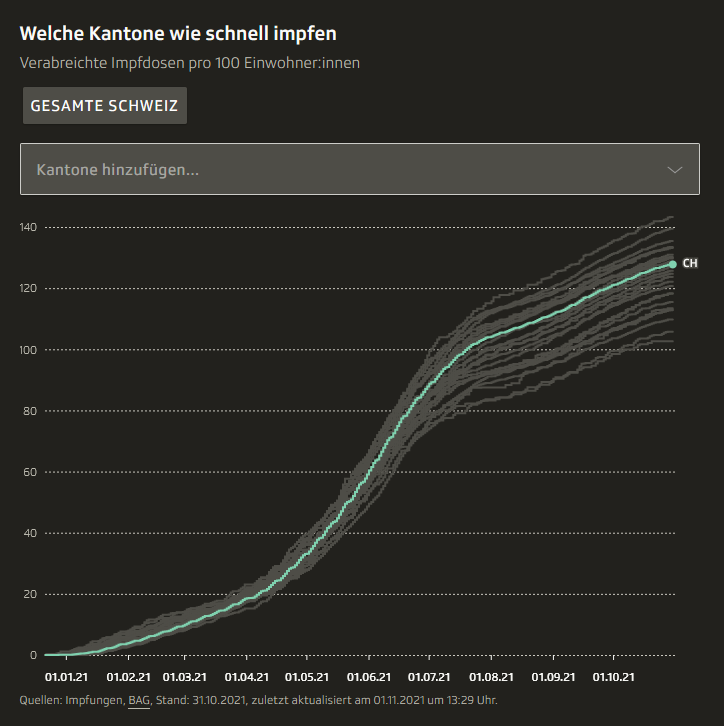
\includegraphics[width=400px]{images/SRF_png1.png}
    \caption{\href{https://www.srf.ch/news/schweiz/impfmonitor-so-impft-die-schweiz-gegen-corona-2}{SRF Impfmonitor}}
    \label{fig:my_label}
\end{figure}

\subsection{Description}
This visualization shows the amount of vaccinations in each canton over time, with the user able to select which data they'd like to be highlighted by either hovering or selecting a canton from a dropdown list.
\subsection{Principles for good design}
\subsubsection{Discoverability}
As you hover over the visualisation, different cantons become highlighted. As most users are likely to move their mouse cursor across the site while browsing, it's likely they will discover this feature of the graph. This means that this graph has very good discoverability.
\subsubsection{Feedback}
On the browsers that we tested, the graph was consistently lagging behind the mouse cursor. This constitutes bad feedback, since while the user is dragging their mouse over the graph, the graph is highlighting data lines approximately half a second after they're hovered over, which makes the visualisation confusing when not moving the cursor very slowly. Otherwise, the visualisation responds to user input almost immediately.
\subsubsection{Affordances}
The Visualization affords the user the ability to select a canton, which will be highlighted in the visualization. 
\subsubsection{Signifiers}
The currently selected data is highlighted. since all non-selected datasets are greyed out, the currently selected data is very easily distinguishable from non-selected data. The selected cantons are also displayed in a list above the Visualisation.
¨\subsubsection{Constraints}
The user is constrained by the selection of cantons. The constraints of the visualization are not optimal, as a user can enter whatever text they want into the canton input box, even text that does not correspond to a canton. this simply leaves the list of cantons in the search query empty. The addition of a text box or overlay informing the user that they have entered an incorrect canton may help improve this aspect of the visualisation.
\subsection{Information Visualisation Principles}
\subsubsection{Elementary Graphical Perception (Cleveland and McGill)}
The visualization uses angle and slope to represents its data, which are not optimal as choices. 
\subsubsection{Information Visualization Principles (Edward Tufte)}
\textbf{Graphical Excellence}
This visualization fails to fulfill Tufte's principle of graphical Excellence. From ca. 01.01.2021 to 01.03.2021 in the graphic, it is nearly impossible to differentiate between the different datasets, even if they are highlighted. this could be fixed by coloring the different cantons in more distinguishable colors, are increasing the scale of the graphic.
\\
\textbf{Tufte's Principles of Data Graphics}
This Visualization has a very low amount of non-data ink. It could be argued that the showing of the greyed-out datasets isn't necessarily helpful, but overall the graphic is very rich in information
\subsection{Interaction Models}
\subsubsection{Seven Stage Model}
\begin{itemize}
    \item \textbf{Goal: } View the vaccination data over time for the canton of Bern 
    \item \textbf{Forming the intention: } The user sees the Visualization on the SRF Impfmonitor and decides to look at the data for Bern 
    \item \textbf{Specifying the Action: }Plan to click on the text box to begin entry of the string "Bern" 
    \item\textbf{Executing the Action: }The user clicks on the field "Kantone Hinzufügen" and begins to enter "Bern". As the string gets closer to completion, the list of cantons shrinks until only Bern is left. The user then clicks on Bern and selects the data set. 
    \item \textbf{State of the World: } The Graphic updates to reflect the highlighting of the data set for Bern. 
    \item \textbf{Perceiving the state of the world: }The user sees the new highlighting of the data pertaining to Bern, and the word "Bern" in the list of Displayed Datasets.
\item \textbf{Interpreting the state of the World: } the User sees that the visualization and its signifiers have updated to match their selection
\item \textbf{Evaluation of the Outcome: } The user has achieved their goal of finding out about the vaccination data for the canton of Bern. 
\end{itemize}
In this Interaction, we see that the user can find their desired dataset very quickly. Had the user been looking for a different canton, they might have run into an issue: While analyzing this visualisation, we noted that the list of cantons in the dropdown menu was ordered in a seemingly arbitrary fashion. This does not correspond with most users expectation of listings in these kinds of graphics, which could lead to confusion and longer time
\begin{figure}[h]
    \centering
    \includegraphics[width=200px]{2021-11-08 00_32_27-Impfmonitor - So impft die Schweiz gegen Corona - News - SRF — Mozilla Firefox.png}
    \caption{The default ordering of cantons in the visualisation}
    \label{fig:my_label}
\end{figure}
\newpage

\section{Visualisation 4}
\begin{figure}[h]
    \centering
    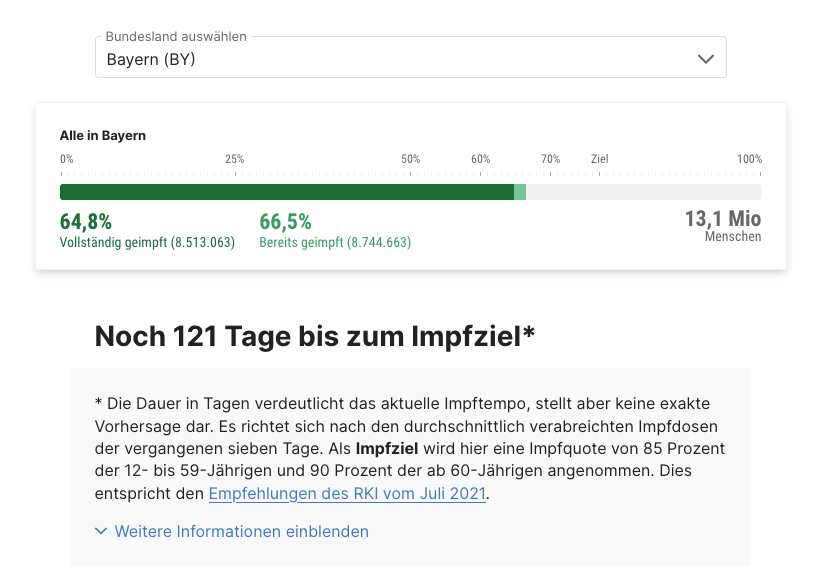
\includegraphics[width=400pt]{images/morgenpost.png}
    \caption{
    \href{https://interaktiv.morgenpost.de/corona-impfungen-deutschland-bundeslaender-weltweit/}{COVID-19 Vaccinations in Germany}}
    \label{fig:my_label}
\end{figure}
\newpage

\subsection{Description}
The above pictured web page shows the vaccination progress in Germany in a couple different ways. One way way, as seen in the visual above is by showing percentages of people fully vaccinated, people vaccinated once and people that are not vaccinated at all, a second way is splitting the population by age groups and federal land and last but not least, a so called "vaccination calendar" but this will be explained in more detail later.
\begin{figure}[h]
    \centering
    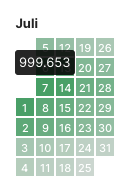
\includegraphics[width=100pt]{images/calendar.png}
    \caption{Vaccination Calendar}
    \label{fig:my_label}
\end{figure}
\subsection{Principles for good design}
\subsubsection{Affordances}
The most prominent affordances on this page are the hyperlinks that are shown as text in a blue font and underlined. As this has been a way of marking hyperlinks for years and on many different pages, it should clearly afford the user to press on them if it picks up the users interest.
\subsubsection{Signifiers}
The page does not provide many signifiers but rather affords the user to discover certain aspects of the page by themselves.  The only major signifier is the description the button to chose from the federal lands.
\subsubsection{Constraints}
The webpage itself is simple and does not allow the user for much interaction except for changing the federal land and/or hovering over dates in the vaccination calendar to see the exact number of vaccines administered on that date which are both logical constraints. The fact that the whole page is in German and the data is only representing the situation inside Germany, might be considered as a cultural constraint as people out side German-speaking areas are generally not able to understand it. 
\subsubsection{Mapping}
The page provides great mapping. Every hyperlink is shown by using a blue font and underlined, there is a scroll bar on the side of the screen to indicate where you are on the page and every clickable object does what it is supposed to.
\subsubsection{Feedback}
The feedback provided on the page is direct and intuitive. Right as the user changes the federal land the user wants to see, the visual immediately changes and as soon as the user hovers over a date on the vaccination calendar, a small drop down menu is visible with the number of vaccinations performed on this date.

\begin{figure}[h]
    \centering
    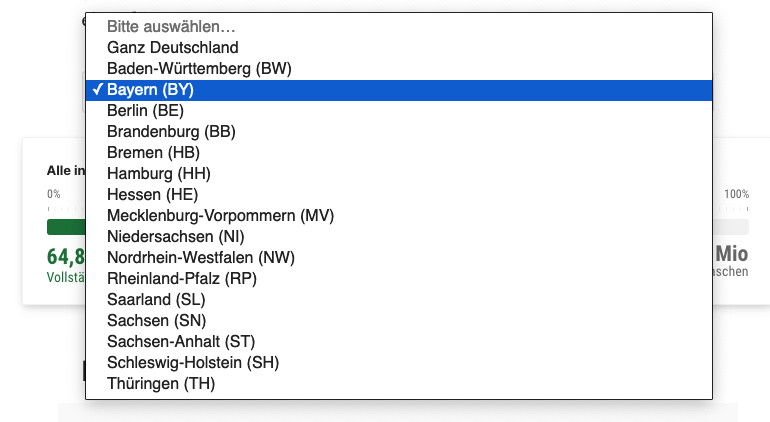
\includegraphics[width=250pt]{images/dropdown.png}
    \caption{Dropdown menu}
    \label{fig:my_label}
\end{figure}

\subsubsection{Discoverability}
Affordances are mainly intuitive or are labeled as such, assisting the user in navigating and exploiting the visualization's capabilities. The visualization, when combined with the fast feedback, results in strong discoverability. It would be easier to find parts that aren't mentioned in the table of contents if there were explicit signifiers for them.

\subsection{Information Visualisation Principles}
\subsubsection{Tufte's Principles for Data Graphics}
Morgenposts visualization shows the data in a small area while still being able to make the large amounts of data coherent and have a reasonable description and tabulation. With the clear use of labeling the visualization makes sure that the user can focus on whats important without having to read a long tutorial on how to use each part of the page. The way that the data is split into different criteria helps revealing the data in different levels and also helps to create a broad overview of the general situation.
With all these points mentioned, we can clearly state that the visual follows Tufte's Principles for graphical excellence.

Regarding the principles for graphical integrity are directly proportional to the quantities as the visualization uses percentages (start of the graph equals 0 percent and end 100). The labeling is clear and makes sure that it does not obstruct any of the important parts of the visualization.

\subsection{Interaction Models}
\subsubsection{Seven stage model}
\begin{itemize}
    \item\textbf{Goal:}
    Find out the number of vaccinations on a specific date.
    \item\textbf{Forming the Intention:}
    Visit Morgenposts interactive page and scroll down to the vaccination calendar.
    \item\textbf{Specifying the Action:}
    Devise a plan to visit Morgenposts interactive page and scroll down to the vaccination calendar.
    \item\textbf{Executing the action:}
    Open your preferred browser, enter the URL to visit the page, scroll down until you see the vaccination calendar and then hover over the date you want more information on.
    \item\textbf{State of the World:}
    The web page loads and displays the data and shows the information.
    \item\textbf{Perceiving the State of the World:}
    User sees that the web page displays the wanted data.
    \item\textbf{Interpreting the State of the World:}
    User determines that the page has successfully loaded all the data and is able to read up on it.
    \item\textbf{Evaluation the Outcome:}
    User decides that the original goal of looking up the number of vaccinations on a specific date has been successfully achieved.
\end{itemize}
\newpage

\section{Identifying a User Goal}
\subsection{Goal Description}
We want to define the user goal as follows: The user wants to find out about the general progress of vaccination in the Federal State of Bavaria, Germany. In the following parts of this assignment we will further describe how the progress of reaching the goal is in two visualizations that we have chosen. To then come to a conclusion we will compare the two pages and assess which one of them has a better experience for the user.
\subsection{Assessment of Visualisation 2 for User Goal}
The first thing the user sees when arriving on the Impfdashboard page is the current vaccination status in large lettering, as well as a smaller header revealing the existence of more content on the page. the site provides great discoverability for this process, as every time a content element is fully visible, the next one is also shown at the bottom of the page, prompting the user to explore further. The user may stop to look at the vaccine clock, after which the next section is "Vaccination Progress by Federal Land". Here, the user may either hover over the map, showing an additional signifier for Bavaria in the second graphic, or hover over Bavaria in the second graphic, showing an additional signifier on the map. The user can now switch to another data set by selecting either "People fully vaccinated" or "Vaccine doses administered" to view different data sets. Overall, the website and this visualization makes it easy for the user to find the data they are looking for, since it offers multiple different ways of viewing the data.

\subsection{Assessment of Visualisation 4 for User Goal}
As soon as the user reaches the landing page of Morgenpost regarding the COVID vaccine, the user will first see some general numbers regarding the vaccination progress in the whole of Germany. A bit further down there is a small table of content where the user is prompted to press on the subsection the user wants to go to. In our case the user would realize that the wanted information cannot be reached through that table of contents and the user is hence prompted to scroll down a bit until the drop down menu is visible that affords the user to chose a Federal State - this is where the user will chose Bavaria and immediately see the current state of the vaccines as soon as the graphic updates. If the user is not satisfied with the data shown in the first visual, the user may scroll down further for two other sets of data. Firstly the distribution of vaccinations in different age groups. The only thing that is expected from the user to know beforehand or find out, is the shortcut for Bavaria. Secondly right underneath the vaccination calendar there is also the amount of vaccinations left per Federal Land per Brand of vaccine.
\newpage
\subsection{Comparison of Visualisations for the User Goal}
Both websites are generally easy to use and therefore its also easy to achieve the goal in both of the websites. Using the KLM model we will calculate for long it takes to reach the goal with that number we will be able to see which websites, even though both are easy to use, is the quicker to achieve the goal.\newline
\newline
\textbf{Impfdashboard: }\newline
- Scroll\tab3.96s\newline
- Point Cursor to Bavaria\tab1.10s\newline
- Click "People Fully Vaccinated"\tab0.10s\newline
- Point Cursor to Bavaria\tab1.10s\newline
- Click "Vaccine Doses administered"\tab0.10s\newline
- Point Cursor to Bavaria\tab1.10s\newline
Total:\tab7.46s
\newline
\newline
\textbf{Morgenpost: }\newline
- Scroll\tab3.96s\newline
- Point Cursor to selection menu\tab1.10s\newline
- Click the menu\tab0.10s\newline
- Click "Bavaria"\tab0.10s\newline
Total:\tab5.26s
\newline
\newline
With this brief analysis we can clearly see that the way that Morgenpost set up their visuals in a bundled way in contrast to Impfdashboards multi-leveled interactivity can save 2.20 seconds but the user would still be able to get the same information. Depending on what level of detail the user wants to have about the data, the time may vary but in our opinion most of the users would follow these steps to get the information.\newline
Further, while using and analyzing those two pages, we found that using Impfdashboard is better because the playful and more in-depth interactivity of the page keeps the user more focused and ready to try out all the features, whereas Morgenpost tries to convey the information in a more efficient and compact way. Depending on how much time you have to find the information the decision of which website to use changes.
\end{document}
